\documentclass[12pt]{article}

%packages
%\usepackage{latexsym}
\usepackage{graphicx}
\usepackage{color}
\usepackage{amsmath}
%\usepackage{dsfont}
\usepackage{placeins}
\usepackage{amssymb}
\usepackage{wasysym}
\usepackage{abstract}
\usepackage{hyperref}

%\usepackage{pstricks,pst-node,pst-tree}

%\usepackage{algpseudocode}
%\usepackage{amsthm}
%\usepackage{hyperref}
%\usepackage{mathrsfs}
%\usepackage{amsfonts}
%\usepackage{bbding}
%\usepackage{listings}
%\usepackage{appendix}
\usepackage[margin=1in]{geometry}
%\geometry{papersize={8.5in,11in},total={6.5in,9in}}
%\usepackage{cancel}
%\usepackage{algorithmic, algorithm}

\newcounter{probnum}
\setcounter{probnum}{1}

%create definition to allow local margin changes
\def\changemargin#1#2{\list{}{\rightmargin#2\leftmargin#1}\item[]}
\let\endchangemargin=\endlist 

%allow equations to span multiple pages
\allowdisplaybreaks

%define colors and color typesetting conveniences
\definecolor{gray}{rgb}{0.5,0.5,0.5}
\definecolor{black}{rgb}{0,0,0}
\definecolor{white}{rgb}{1,1,1}
\definecolor{blue}{rgb}{0.5,0.5,1}
\newcommand{\inblue}[1]{\color{blue}#1 \color{black}}
\definecolor{green}{rgb}{0.133,0.545,0.133}
\newcommand{\ingreen}[1]{\color{green}#1 \color{black}}
\definecolor{yellow}{rgb}{1,0.549,0}
\newcommand{\inyellow}[1]{\color{yellow}#1 \color{black}}
\definecolor{red}{rgb}{1,0.133,0.133}
\newcommand{\inred}[1]{\color{red}#1 \color{black}}
\definecolor{purple}{rgb}{0.58,0,0.827}
\newcommand{\inpurple}[1]{\color{purple}#1 \color{black}}
\definecolor{backgcode}{rgb}{0.97,0.97,0.8}
\definecolor{Brown}{cmyk}{0,0.81,1,0.60}
\definecolor{OliveGreen}{cmyk}{0.64,0,0.95,0.40}
\definecolor{CadetBlue}{cmyk}{0.62,0.57,0.23,0}

%define new math operators
\DeclareMathOperator*{\argmax}{arg\,max~}
\DeclareMathOperator*{\argmin}{arg\,min~}
\DeclareMathOperator*{\argsup}{arg\,sup~}
\DeclareMathOperator*{\arginf}{arg\,inf~}
\DeclareMathOperator*{\convolution}{\text{\Huge{$\ast$}}}
\newcommand{\infconv}[2]{\convolution^\infty_{#1 = 1} #2}
%true functions

%%%% GENERAL SHORTCUTS

%shortcuts for pure typesetting conveniences
\newcommand{\bv}[1]{\boldsymbol{#1}}

%shortcuts for compound constants
\newcommand{\BetaDistrConst}{\dfrac{\Gamma(\alpha + \beta)}{\Gamma(\alpha)\Gamma(\beta)}}
\newcommand{\NormDistrConst}{\dfrac{1}{\sqrt{2\pi\sigma^2}}}

%shortcuts for conventional symbols
\newcommand{\tsq}{\tau^2}
\newcommand{\tsqh}{\hat{\tau}^2}
\newcommand{\sigsq}{\sigma^2}
\newcommand{\sigsqsq}{\parens{\sigma^2}^2}
\newcommand{\sigsqovern}{\dfrac{\sigsq}{n}}
\newcommand{\tausq}{\tau^2}
\newcommand{\tausqalpha}{\tau^2_\alpha}
\newcommand{\tausqbeta}{\tau^2_\beta}
\newcommand{\tausqsigma}{\tau^2_\sigma}
\newcommand{\betasq}{\beta^2}
\newcommand{\sigsqvec}{\bv{\sigma}^2}
\newcommand{\sigsqhat}{\hat{\sigma}^2}
\newcommand{\sigsqhatmlebayes}{\sigsqhat_{\text{Bayes, MLE}}}
\newcommand{\sigsqhatmle}[1]{\sigsqhat_{#1, \text{MLE}}}
\newcommand{\bSigma}{\bv{\Sigma}}
\newcommand{\bSigmainv}{\bSigma^{-1}}
\newcommand{\thetavec}{\bv{\theta}}
\newcommand{\thetahat}{\hat{\theta}}
\newcommand{\thetahatmle}{\hat{\theta}_{\mathrm{MLE}}}
\newcommand{\thetavechatmle}{\hat{\thetavec}_{\mathrm{MLE}}}
\newcommand{\muhat}{\hat{\mu}}
\newcommand{\musq}{\mu^2}
\newcommand{\muvec}{\bv{\mu}}
\newcommand{\muhatmle}{\muhat_{\text{MLE}}}
\newcommand{\lambdahat}{\hat{\lambda}}
\newcommand{\lambdahatmle}{\lambdahat_{\text{MLE}}}
\newcommand{\etavec}{\bv{\eta}}
\newcommand{\alphavec}{\bv{\alpha}}
\newcommand{\minimaxdec}{\delta^*_{\mathrm{mm}}}
\newcommand{\ybar}{\bar{y}}
\newcommand{\xbar}{\bar{x}}
\newcommand{\Xbar}{\bar{X}}
\newcommand{\iid}{~{\buildrel iid \over \sim}~}
\newcommand{\inddist}{~{\buildrel ind \over \sim}~}
\newcommand{\approxdist}{~{\buildrel approx \over \sim}~}
\newcommand{\equalsindist}{~{\buildrel d \over =}~}
\newcommand{\loglik}[1]{\ell\parens{#1}}
\newcommand{\thetahatkminone}{\thetahat^{(k-1)}}
\newcommand{\thetahatkplusone}{\thetahat^{(k+1)}}
\newcommand{\thetahatk}{\thetahat^{(k)}}
\newcommand{\half}{\frac{1}{2}}
\newcommand{\third}{\frac{1}{3}}
\newcommand{\twothirds}{\frac{2}{3}}
\newcommand{\fourth}{\frac{1}{4}}
\newcommand{\fifth}{\frac{1}{5}}
\newcommand{\sixth}{\frac{1}{6}}

%shortcuts for vector and matrix notation
\newcommand{\A}{\bv{A}}
\newcommand{\At}{\A^T}
\newcommand{\Ainv}{\inverse{\A}}
\newcommand{\B}{\bv{B}}
\newcommand{\K}{\bv{K}}
\newcommand{\Kt}{\K^T}
\newcommand{\Kinv}{\inverse{K}}
\newcommand{\Kinvt}{(\Kinv)^T}
\newcommand{\M}{\bv{M}}
\newcommand{\Bt}{\B^T}
\newcommand{\Q}{\bv{Q}}
\newcommand{\Qt}{\Q^T}
\newcommand{\R}{\bv{R}}
\newcommand{\Rt}{\R^T}
\newcommand{\Z}{\bv{Z}}
\newcommand{\X}{\bv{X}}
\newcommand{\Xsub}{\X_{\text{(sub)}}}
\newcommand{\Xsubadj}{\X_{\text{(sub,adj)}}}
\newcommand{\I}{\bv{I}}
\newcommand{\Y}{\bv{Y}}
\newcommand{\sigsqI}{\sigsq\I}
\renewcommand{\P}{\bv{P}}
\newcommand{\Psub}{\P_{\text{(sub)}}}
\newcommand{\Pt}{\P^T}
\newcommand{\Pii}{P_{ii}}
\newcommand{\Pij}{P_{ij}}
\newcommand{\IminP}{(\I-\P)}
\newcommand{\Xt}{\bv{X}^T}
\newcommand{\XtX}{\Xt\X}
\newcommand{\XtXinv}{\parens{\Xt\X}^{-1}}
\newcommand{\XtXinvXt}{\XtXinv\Xt}
\newcommand{\XXtXinvXt}{\X\XtXinvXt}
\newcommand{\x}{\bv{x}}
\newcommand{\onevec}{\bv{1}}
\newcommand{\oneton}{1, \ldots, n}
\newcommand{\yoneton}{y_1, \ldots, y_n}
\newcommand{\yonetonorder}{y_{(1)}, \ldots, y_{(n)}}
\newcommand{\Yoneton}{Y_1, \ldots, Y_n}
\newcommand{\iinoneton}{i \in \braces{\oneton}}
\newcommand{\onetom}{1, \ldots, m}
\newcommand{\jinonetom}{j \in \braces{\onetom}}
\newcommand{\xoneton}{x_1, \ldots, x_n}
\newcommand{\Xoneton}{X_1, \ldots, X_n}
\newcommand{\xt}{\x^T}
\newcommand{\y}{\bv{y}}
\newcommand{\yt}{\y^T}
\renewcommand{\c}{\bv{c}}
\newcommand{\ct}{\c^T}
\newcommand{\tstar}{\bv{t}^*}
\renewcommand{\u}{\bv{u}}
\renewcommand{\v}{\bv{v}}
\renewcommand{\a}{\bv{a}}
\newcommand{\s}{\bv{s}}
\newcommand{\yadj}{\y_{\text{(adj)}}}
\newcommand{\xjadj}{\x_{j\text{(adj)}}}
\newcommand{\xjadjM}{\x_{j \perp M}}
\newcommand{\yhat}{\hat{\y}}
\newcommand{\yhatsub}{\yhat_{\text{(sub)}}}
\newcommand{\yhatstar}{\yhat^*}
\newcommand{\yhatstarnew}{\yhatstar_{\text{new}}}
\newcommand{\z}{\bv{z}}
\newcommand{\zt}{\z^T}
\newcommand{\bb}{\bv{b}}
\newcommand{\bbt}{\bb^T}
\newcommand{\bbeta}{\bv{\beta}}
\newcommand{\beps}{\bv{\epsilon}}
\newcommand{\bepst}{\beps^T}
\newcommand{\e}{\bv{e}}
\newcommand{\Mofy}{\M(\y)}
\newcommand{\KofAlpha}{K(\alpha)}
\newcommand{\ellset}{\mathcal{L}}
\newcommand{\oneminalph}{1-\alpha}
\newcommand{\SSE}{\text{SSE}}
\newcommand{\SSEsub}{\text{SSE}_{\text{(sub)}}}
\newcommand{\MSE}{\text{MSE}}
\newcommand{\RMSE}{\text{RMSE}}
\newcommand{\SSR}{\text{SSR}}
\newcommand{\SST}{\text{SST}}
\newcommand{\JSest}{\delta_{\text{JS}}(\x)}
\newcommand{\Bayesest}{\delta_{\text{Bayes}}(\x)}
\newcommand{\EmpBayesest}{\delta_{\text{EmpBayes}}(\x)}
\newcommand{\BLUPest}{\delta_{\text{BLUP}}}
\newcommand{\MLEest}[1]{\hat{#1}_{\text{MLE}}}

%shortcuts for Linear Algebra stuff (i.e. vectors and matrices)
\newcommand{\twovec}[2]{\bracks{\begin{array}{c} #1 \\ #2 \end{array}}}
\newcommand{\threevec}[3]{\bracks{\begin{array}{c} #1 \\ #2 \\ #3 \end{array}}}
\newcommand{\fivevec}[5]{\bracks{\begin{array}{c} #1 \\ #2 \\ #3 \\ #4 \\ #5 \end{array}}}
\newcommand{\twobytwomat}[4]{\bracks{\begin{array}{cc} #1 & #2 \\ #3 & #4 \end{array}}}
\newcommand{\threebytwomat}[6]{\bracks{\begin{array}{cc} #1 & #2 \\ #3 & #4 \\ #5 & #6 \end{array}}}

%shortcuts for conventional compound symbols
\newcommand{\thetainthetas}{\theta \in \Theta}
\newcommand{\reals}{\mathbb{R}}
\newcommand{\complexes}{\mathbb{C}}
\newcommand{\rationals}{\mathbb{Q}}
\newcommand{\integers}{\mathbb{Z}}
\newcommand{\naturals}{\mathbb{N}}
\newcommand{\forallninN}{~~\forall n \in \naturals}
\newcommand{\forallxinN}[1]{~~\forall #1 \in \reals}
\newcommand{\matrixdims}[2]{\in \reals^{\,#1 \times #2}}
\newcommand{\inRn}[1]{\in \reals^{\,#1}}
\newcommand{\mathimplies}{\quad\Rightarrow\quad}
\newcommand{\mathlogicequiv}{\quad\Leftrightarrow\quad}
\newcommand{\eqncomment}[1]{\quad \text{(#1)}}
\newcommand{\limitn}{\lim_{n \rightarrow \infty}}
\newcommand{\limitN}{\lim_{N \rightarrow \infty}}
\newcommand{\limitd}{\lim_{d \rightarrow \infty}}
\newcommand{\limitt}{\lim_{t \rightarrow \infty}}
\newcommand{\limitsupn}{\limsup_{n \rightarrow \infty}~}
\newcommand{\limitinfn}{\liminf_{n \rightarrow \infty}~}
\newcommand{\limitk}{\lim_{k \rightarrow \infty}}
\newcommand{\limsupn}{\limsup_{n \rightarrow \infty}}
\newcommand{\limsupk}{\limsup_{k \rightarrow \infty}}
\newcommand{\floor}[1]{\left\lfloor #1 \right\rfloor}
\newcommand{\ceil}[1]{\left\lceil #1 \right\rceil}

%shortcuts for environments
\newcommand{\beqn}{\vspace{-0.25cm}\begin{eqnarray*}}
\newcommand{\eeqn}{\end{eqnarray*}}
\newcommand{\bneqn}{\vspace{-0.25cm}\begin{eqnarray}}
\newcommand{\eneqn}{\end{eqnarray}}

%shortcuts for mini environments
\newcommand{\parens}[1]{\left(#1\right)}
\newcommand{\squared}[1]{\parens{#1}^2}
\newcommand{\tothepow}[2]{\parens{#1}^{#2}}
\newcommand{\prob}[1]{\mathbb{P}\parens{#1}}
\newcommand{\littleo}[1]{o\parens{#1}}
\newcommand{\bigo}[1]{O\parens{#1}}
\newcommand{\Lp}[1]{\mathbb{L}^{#1}}
\renewcommand{\arcsin}[1]{\text{arcsin}\parens{#1}}
\newcommand{\prodonen}[2]{\bracks{\prod_{#1=1}^n #2}}
\newcommand{\mysum}[4]{\sum_{#1=#2}^{#3} #4}
\newcommand{\sumonen}[2]{\sum_{#1=1}^n #2}
\newcommand{\infsum}[2]{\sum_{#1=1}^\infty #2}
\newcommand{\infprod}[2]{\prod_{#1=1}^\infty #2}
\newcommand{\infunion}[2]{\bigcup_{#1=1}^\infty #2}
\newcommand{\infinter}[2]{\bigcap_{#1=1}^\infty #2}
\newcommand{\infintegral}[2]{\int^\infty_{-\infty} #2 ~\text{d}#1}
\newcommand{\supthetas}[1]{\sup_{\thetainthetas}\braces{#1}}
\newcommand{\bracks}[1]{\left[#1\right]}
\newcommand{\braces}[1]{\left\{#1\right\}}
\newcommand{\set}[1]{\left\{#1\right\}}
\newcommand{\abss}[1]{\left|#1\right|}
\newcommand{\norm}[1]{\left|\left|#1\right|\right|}
\newcommand{\normsq}[1]{\norm{#1}^2}
\newcommand{\inverse}[1]{\parens{#1}^{-1}}
\newcommand{\rowof}[2]{\parens{#1}_{#2\cdot}}

%shortcuts for functionals
\newcommand{\realcomp}[1]{\text{Re}\bracks{#1}}
\newcommand{\imagcomp}[1]{\text{Im}\bracks{#1}}
\newcommand{\range}[1]{\text{range}\bracks{#1}}
\newcommand{\colsp}[1]{\text{colsp}\bracks{#1}}
\newcommand{\rowsp}[1]{\text{rowsp}\bracks{#1}}
\newcommand{\tr}[1]{\text{tr}\bracks{#1}}
\newcommand{\rank}[1]{\text{rank}\bracks{#1}}
\newcommand{\proj}[2]{\text{Proj}_{#1}\bracks{#2}}
\newcommand{\projcolspX}[1]{\text{Proj}_{\colsp{\X}}\bracks{#1}}
\newcommand{\median}[1]{\text{median}\bracks{#1}}
\newcommand{\mean}[1]{\text{mean}\bracks{#1}}
\newcommand{\dime}[1]{\text{dim}\bracks{#1}}
\renewcommand{\det}[1]{\text{det}\bracks{#1}}
\newcommand{\expe}[1]{\mathbb{E}\bracks{#1}}
\newcommand{\expeabs}[1]{\expe{\abss{#1}}}
\newcommand{\expesub}[2]{\mathbb{E}_{#1}\bracks{#2}}
\newcommand{\indic}[1]{\mathds{1}_{#1}}
\newcommand{\var}[1]{\mathbb{V}\text{ar}\bracks{#1}}
\newcommand{\sd}[1]{\mathbb{S}\text{D}\bracks{#1}}
\newcommand{\cov}[2]{\text{Cov}\bracks{#1, #2}}
\newcommand{\corr}[2]{\text{Corr}\bracks{#1, #2}}
\newcommand{\se}[1]{\text{SE}\bracks{#1}}
\newcommand{\seest}[1]{\hat{\text{SE}}\bracks{#1}}
\newcommand{\bias}[1]{\text{Bias}\bracks{#1}}
\newcommand{\partialop}[2]{\dfrac{\partial}{\partial #1}\bracks{#2}}
\newcommand{\secpartialop}[2]{\dfrac{\partial^2}{\partial #1^2}\bracks{#2}}
\newcommand{\mixpartialop}[3]{\dfrac{\partial^2}{\partial #1 \partial #2}\bracks{#3}}

%shortcuts for functions
\renewcommand{\exp}[1]{\mathrm{exp}\parens{#1}}
\renewcommand{\cos}[1]{\text{cos}\parens{#1}}
\renewcommand{\sin}[1]{\text{sin}\parens{#1}}
\newcommand{\sign}[1]{\text{sign}\parens{#1}}
\newcommand{\are}[1]{\mathrm{ARE}\parens{#1}}
\newcommand{\natlog}[1]{\ln\parens{#1}}
\newcommand{\oneover}[1]{\frac{1}{#1}}
\newcommand{\overtwo}[1]{\frac{#1}{2}}
\newcommand{\overn}[1]{\frac{#1}{n}}
\newcommand{\oneoversqrt}[1]{\oneover{\sqrt{#1}}}
\newcommand{\sqd}[1]{\parens{#1}^2}
\newcommand{\loss}[1]{\ell\parens{\theta, #1}}
\newcommand{\losstwo}[2]{\ell\parens{#1, #2}}
\newcommand{\cf}{\phi(t)}

%English language specific shortcuts
\newcommand{\ie}{\textit{i.e.} }
\newcommand{\AKA}{\textit{AKA} }
\renewcommand{\iff}{\textit{iff}}
\newcommand{\eg}{\textit{e.g.} }
\newcommand{\st}{\textit{s.t.} }
\newcommand{\wrt}{\textit{w.r.t.} }
\newcommand{\mathst}{~~\text{\st}~~}
\newcommand{\mathand}{~~\text{and}~~}
\newcommand{\ala}{\textit{a la} }
\newcommand{\ppp}{posterior predictive p-value}
\newcommand{\dd}{dataset-to-dataset}

%shortcuts for distribution titles
\newcommand{\logistic}[2]{\mathrm{Logistic}\parens{#1,\,#2}}
\newcommand{\bernoulli}[1]{\mathrm{Bernoulli}\parens{#1}}
\newcommand{\betanot}[2]{\mathrm{Beta}\parens{#1,\,#2}}
\newcommand{\stdbetanot}{\betanot{\alpha}{\beta}}
\newcommand{\multnormnot}[3]{\mathcal{N}_{#1}\parens{#2,\,#3}}
\newcommand{\normnot}[2]{\mathcal{N}\parens{#1,\,#2}}
\newcommand{\classicnormnot}{\normnot{\mu}{\sigsq}}
\newcommand{\stdnormnot}{\normnot{0}{1}}
\newcommand{\uniform}[2]{\mathrm{U}\parens{#1,\,#2}}
\newcommand{\stduniform}{\uniform{0}{1}}
\newcommand{\exponential}[1]{\mathrm{Exp}\parens{#1}}
\newcommand{\gammadist}[2]{\mathrm{Gamma}\parens{#1, #2}}
\newcommand{\poisson}[1]{\mathrm{Poisson}\parens{#1}}
\newcommand{\binomial}[2]{\mathrm{Binomial}\parens{#1,\,#2}}
\newcommand{\rayleigh}[1]{\mathrm{Rayleigh}\parens{#1}}
\newcommand{\multinomial}[2]{\mathrm{Multinomial}\parens{#1,\,#2}}
\newcommand{\gammanot}[2]{\mathrm{Gamma}\parens{#1,\,#2}}
\newcommand{\cauchynot}[2]{\text{Cauchy}\parens{#1,\,#2}}
\newcommand{\invchisqnot}[1]{\text{Inv}\chisq{#1}}
\newcommand{\invscaledchisqnot}[2]{\text{ScaledInv}\ncchisq{#1}{#2}}
\newcommand{\invgammanot}[2]{\text{InvGamma}\parens{#1,\,#2}}
\newcommand{\chisq}[1]{\chi^2_{#1}}
\newcommand{\ncchisq}[2]{\chi^2_{#1}\parens{#2}}
\newcommand{\ncF}[3]{F_{#1,#2}\parens{#3}}

%shortcuts for PDF's of common distributions
\newcommand{\logisticpdf}[3]{\oneover{#3}\dfrac{\exp{-\dfrac{#1 - #2}{#3}}}{\parens{1+\exp{-\dfrac{#1 - #2}{#3}}}^2}}
\newcommand{\betapdf}[3]{\dfrac{\Gamma(#2 + #3)}{\Gamma(#2)\Gamma(#3)}#1^{#2-1} (1-#1)^{#3-1}}
\newcommand{\normpdf}[3]{\frac{1}{\sqrt{2\pi#3}}\exp{-\frac{1}{2#3}(#1 - #2)^2}}
\newcommand{\normpdfvarone}[2]{\dfrac{1}{\sqrt{2\pi}}e^{-\half(#1 - #2)^2}}
\newcommand{\chisqpdf}[2]{\dfrac{1}{2^{#2/2}\Gamma(#2/2)}\; {#1}^{#2/2-1} e^{-#1/2}}
\newcommand{\invchisqpdf}[2]{\dfrac{2^{-\overtwo{#1}}}{\Gamma(#2/2)}\,{#1}^{-\overtwo{#2}-1}  e^{-\oneover{2 #1}}}
\newcommand{\exponentialpdf}[2]{#2\exp{-#2#1}}
\newcommand{\poissonpdf}[2]{\dfrac{e^{-#1} #1^{#2}}{#2!}}
\newcommand{\binomialpdf}[3]{\binom{#2}{#1}#3^{#1}(1-#3)^{#2-#1}}
\newcommand{\rayleighpdf}[2]{\dfrac{#1}{#2^2}\exp{-\dfrac{#1^2}{2 #2^2}}}
\newcommand{\gammapdf}[3]{\dfrac{#3^#2}{\Gamma\parens{#2}}#1^{#2-1}\exp{-#3 #1}}
\newcommand{\cauchypdf}[3]{\oneover{\pi} \dfrac{#3}{\parens{#1-#2}^2 + #3^2}}
\newcommand{\Gammaf}[1]{\Gamma\parens{#1}}

%shortcuts for miscellaneous typesetting conveniences
\newcommand{\notesref}[1]{\marginpar{\color{gray}\tt #1\color{black}}}

%%%% DOMAIN-SPECIFIC SHORTCUTS

%Real analysis related shortcuts
\newcommand{\zeroonecl}{\bracks{0,1}}
\newcommand{\forallepsgrzero}{\forall \epsilon > 0~~}
\newcommand{\lessthaneps}{< \epsilon}
\newcommand{\fraccomp}[1]{\text{frac}\bracks{#1}}

%Bayesian related shortcuts
\newcommand{\yrep}{y^{\text{rep}}}
\newcommand{\yrepisq}{(\yrep_i)^2}
\newcommand{\yrepvec}{\bv{y}^{\text{rep}}}


%Probability shortcuts
\newcommand{\SigField}{\mathcal{F}}
\newcommand{\ProbMap}{\mathcal{P}}
\newcommand{\probtrinity}{\parens{\Omega, \SigField, \ProbMap}}
\newcommand{\convp}{~{\buildrel p \over \rightarrow}~}
\newcommand{\convLp}[1]{~{\buildrel \Lp{#1} \over \rightarrow}~}
\newcommand{\nconvp}{~{\buildrel p \over \nrightarrow}~}
\newcommand{\convae}{~{\buildrel a.e. \over \longrightarrow}~}
\newcommand{\convau}{~{\buildrel a.u. \over \longrightarrow}~}
\newcommand{\nconvau}{~{\buildrel a.u. \over \nrightarrow}~}
\newcommand{\nconvae}{~{\buildrel a.e. \over \nrightarrow}~}
\newcommand{\convd}{~{\buildrel \mathcal{D} \over \rightarrow}~}
\newcommand{\nconvd}{~{\buildrel \mathcal{D} \over \nrightarrow}~}
\newcommand{\withprob}{~~\text{w.p.}~~}
\newcommand{\io}{~~\text{i.o.}}

\newcommand{\Acl}{\bar{A}}
\newcommand{\ENcl}{\bar{E}_N}
\newcommand{\diam}[1]{\text{diam}\parens{#1}}

\newcommand{\taua}{\tau_a}

\newcommand{\myint}[4]{\int_{#2}^{#3} #4 \,\text{d}#1}
\newcommand{\laplacet}[1]{\mathscr{L}\bracks{#1}}
\newcommand{\laplaceinvt}[1]{\mathscr{L}^{-1}\bracks{#1}}
\renewcommand{\min}[1]{\text{min}\braces{#1}}

\newcommand{\Vbar}[1]{\bar{V}\parens{#1}}
\newcommand{\expnegrtau}{\exp{-r\tau}}

%%% problem typesetting
\newcommand{\problem}{\vspace{0.2cm} \noindent {\large{\textsf{Problem \arabic{probnum}~}}} \addtocounter{probnum}{1}}
%\newcommand{\easyproblem}{\ingreen{\noindent \textsf{Problem \arabic{probnum}~}} \addtocounter{probnum}{1}}
%\newcommand{\intermediateproblem}{\noindent \inyellow{\textsf{Problem \arabic{probnum}~}} \addtocounter{probnum}{1}}
%\newcommand{\hardproblem}{\inred{\noindent \textsf{Problem \arabic{probnum}~}} \addtocounter{probnum}{1}}
%\newcommand{\extracreditproblem}{\noindent \inpurple{\textsf{Problem \arabic{probnum}~}} \addtocounter{probnum}{1}}

\newcommand{\easysubproblem}{\ingreen{\item}}
\newcommand{\intermediatesubproblem}{\inyellow{\item}}
\newcommand{\hardsubproblem}{\inred{\item}}
\newcommand{\extracreditsubproblem}{\inpurple{\item}}
\renewcommand{\labelenumi}{(\alph{enumi})}


\title{Statistics 101 Summer I 2011 \\ Homework \#4}
\author{Adam Kapelner, Instructor}

\date{Due noon, Friday, June 24, 2011 (in my mail slot)}

\renewcommand{\abstractname}{Instructions and Philosophy}

\begin{document}
\maketitle


\begin{abstract}
Copy the previous first paragraph and tack on the following: reviewing lecture notes from class is really important.

In Stine \& Foster, read chapter 15, 16 carefully, then chapter 5 (ignore the section on Cramer's $V$), then chapter 18. You can ignore the subsections on skewness and kurtosis and the SRS condition with $n$ being 10\% of $N$ (since we view $N \approx \infty$ anyway). I also recommend reading Wikipedia's article on \href{http://en.wikipedia.org/wiki/Simpson%27s_paradox}{Simpson's Paradox}.

Once again, \ingreen{green} means \textit{easy}, \inyellow{yellow} means \textit{intermediate}, \inred{red} means \textit{difficult}, and \inpurple{purple} means \textit{extra credit}. This homework is worth 100 points but the point distribution will not be determined until after the due date. Late homework will be penalized 10 points per day. Beyond Monday, June 27 at 9AM, it will receive a zero. 15 points are given as a bonus if the homework is typed using \LaTeX ~(please comment out or delete all extraneous text).
\end{abstract}

\paragraph{Distribution Theory} In this section we will learn about the most important distributions used for testing in the field of Statistics. \\

\problem We're going to learn more about the CLT and its cousin, the $T$ distribution. We will use the notation $T_{df}$ for a $T$ distribution with $df$ degrees of freedom and the usual $Z = \stdnormnot$. The notation $\convd$ means as $\limitn$ the PDF's become equal; the notation $\equalsindist$ means the PDF's are exactly equal right now \ie at any $n$. $S_n$ will refer to the r.v. that is the sum of $\Xoneton$ as usual, but $\sddist$ is the r.v. that represents the distribution that $s$, the sample standard deviation, is drawn from. In other words:

\beqn
\sddist = \sqrt{\oneover{n-1}\sumonen{i}{\squared{X_i - \Xbar}}}
\eeqn

This distribution is immensely complicated and non-standard. It would take PhD's a good few days of \href{http://en.wikipedia.org/wiki/User:Rb88guy/sandbox}{computations and algebra} to familiarize themselves with its properties.

\benum
\easysubproblem Show the following by invoking the CLT from class and using shifts and scales:

\beqn
\Xoneton \iid \text{(any PMF or PDF with mean $\mu$ and std dev $\sigma$)}, \quad \frac{\sqrt{n}\parens{\Xbar - \mu}}{\sigma} \convd Z
\eeqn

\easysubproblem Show the following by invoking the CLT from class and using shifts and scales:

\beqn
\Xoneton \iid \text{(any PMF or PDF with mean $\mu$ and std dev $\sigma$)}, \quad \frac{\parens{S_n - n\mu}}{\sqrt{n}\sigma} \convd Z
\eeqn

\easysubproblem Explain why the following is \textit{not} true:

\beqn
\Xoneton \iid \text{(any PMF or PDF with mean $\mu$ and std dev $\sigma$)} \mathimplies \frac{\parens{\Xbar - \mu}}{\frac{\sigma}{\sqrt{n}}} \equalsindist Z
\eeqn

\intermediatesubproblem Explain why the following is \textit{not} true. Be sure to look in your notes; there are two things wrong here.

\beqn
\Xoneton \iid \text{(any PMF or PDF with mean $\mu$ and std dev $\sigma$)} \mathimplies \frac{\parens{\Xbar - \mu}}{\frac{\sigma}{\sqrt{n}}} \equalsindist T_{n-1}
\eeqn

\intermediatesubproblem Explain why the following is \textit{not} true. Be sure to look in your notes.

\beqn
\Xoneton \iid \text{(any PMF or PDF with mean $\mu$ and std dev $\sigma$)} \mathimplies \frac{\parens{\Xbar - \mu}}{\frac{\sddist}{\sqrt{n}}} \equalsindist T_{n-1}
\eeqn

\hardsubproblem Explain why the following \textit{is} true:

\beqn
\Xoneton \iid \normnot{\mu}{\sigsq} \mathimplies \frac{\parens{\Xbar - \mu}}{\frac{\sigma}{\sqrt{n}}} \equalsindist Z
\eeqn

\easysubproblem Is the following true?

\beqn
\Xoneton \iid \normnot{\mu}{\sigsq} \mathimplies \frac{\parens{\Xbar - \mu}}{\frac{\sddist}{\sqrt{n}}} \equalsindist T_{n-1}
\eeqn

What is the critical premise most people leave out (even S\&F) when claiming their test statistic is $T$-distributed?
\eenum

\problem We talk a lot about how the $T_{df}$ converges to a $Z$ as the degrees of freedom (df) gets larger. The ballpark approximation we gave in class was that $df \geq 29$, we call it a day. We're going to see just how close this approximation is.

\benum
\easysubproblem Run the following code in \texttt{R}:

\footnotesize
\begin{verbatim}
x = seq(-6, 6, 0.01);
plot(x, dt(x, 1), 
  type = "l", 
  col = "chocolate", 
  ylim = c(0, 0.39), 
  ylab = "prob density", 
  xlab = "t (or z)", 
  main = "The T distribution as an approximation\nto the Z distribution");
lines(x, dt(x, 5), type = "l", col = "blue");
lines(x, dt(x, 10), type = "l", col = "green");
lines(x, dt(x, 20), type = "l", col = "yellow");
lines(x, dt(x, 30), type = "l", col = "brown");
lines(x, dt(x, 50), type = "l", col = "purple");
lines(x, dt(x, 100), type = "l", col = "gray");
lines(x, dnorm(x), type = "l", col = "red");
#placeholder for last line
\end{verbatim}
\normalsize

The code will graph the PDF of $T_1$ in ``chocolate'' color, the PDF of $T_5$ in blue, the PDF of $T_{10}$ green, the PDF of $T_{20}$ in yellow, the PDF of $T_{30}$ in brown, the PDF of $T_{50}$ in purple, the PDF of $T_{100}$ in gray, and the PDF of the $Z = \stdnormnot$ in red. \\

What happens as the degrees of freedom gets larger?

\intermediatesubproblem Now we're going to run the same code again, but this time we're only going to plot the right tail \ie the portion from $z=1.96$ (your favorite number) and greater:

\footnotesize
\begin{verbatim}
x = seq(1.96, 3, 0.001);
plot(x, dt(x, 1), 
  pch = ".", 
  col = "chocolate", 
  ylim = c(0, 0.07), xlim = c(1.96, 3),
  ylab = "prob density", 
  xlab = "t (or z)", 
  main = "The T distribution as an approximation\nto the Z distribution");
lines(x, dt(x, 5), pch = ".", col = "blue");
lines(x, dt(x, 10), pch = ".", col = "green");
lines(x, dt(x, 20), pch = ".", col = "yellow");
lines(x, dt(x, 30), pch = ".", col = "brown");
lines(x, dt(x, 50), pch = ".", col = "purple");
lines(x, dt(x, 100), pch = ".", col = "gray");
lines(x, dnorm(x), pch = ".", col = "red");
#placeholder for last line
\end{verbatim}
\normalsize

Maximize the plot window (make the graphic as big as you can). Estimate what percent our approximation is off when we use $z_{0.025}$ instead of $t_{0.025, 30}$ by looking at the plot. Is this large enough to care under quotidian circumstances? 

\intermediatesubproblem Estimate what percent the approximation would be off when you use $z_{0.025}$ instead of $t_{0.025, 100}$ by looking at the plot.

\extracreditsubproblem In one of the lectures, I wrote on the board that the limit of a $T$ as its $df$ (which we will denote $\nu$ for this problem) increases is a $Z$:

\beqn
\lim_{\nu \rightarrow \infty} T_{\nu} = Z
\eeqn 

For persnikety mathematicians, this is an inexact statement because limits aren't defined for r.v.'s, only for their densities.\footnote{This is also inexact, but to find out why, you're going to have to enroll in the PhD program.} The following is the density function (the PDF) for the $T$ distribution with $\nu$ degrees of freedom:

\beqn
f_{T_\nu}(x) = \frac{\Gamma(\frac{\nu+1}{2})} {\sqrt{\nu\pi}\,\Gamma(\frac{\nu}{2})} \parens{1+\frac{x^2}{\nu}}^{-\parens{\frac{\nu+1}{2}}}
\eeqn

Prove that the density of the $T$ distribution (above) converges to the density of the $Z$ distribution (which is in your notes) for all values of $x$. Proving this will constitute a more mathematically precise statement and will corroborate the picture you see in parts (a) and (b). \\

I will give you two hints. One: assume the following is true without proof:

\beqn
\lim_{\nu \rightarrow \infty} \frac{\Gamma(\frac{\nu+1}{2})}{\sqrt{\nu}\,\Gamma(\frac{\nu}{2})} = \oneoversqrt{2}
\eeqn

If I didn't give you the above, you would've needed tons of tricks and intimate knowledge of the \href{http://en.wikipedia.org/wiki/Gamma_function}{gamma function} (which I explained briefly at the end of one of the lectures) to prove and it's a couple pages of algebra. Two: review the tricks we used during the derivation of the Poisson PMF from the Binomial PMF which is in your notes.

\extracreditsubproblem Why is the $t$-test called ``Student's $t$-test''? Tell the story of the $T$ distribution.
\eenum 


\problem This problem will ask basic questions about the $\chisq{df}$ distribution in order to familiarize you with it.

\benum
\easysubproblem Write the definition of the $\chisq{df}$ r.v. as we did in class.
\easysubproblem Use the table from the book (p.743) which I handed out in class to approximate how much density there is in the $\chisq{4}$ PDF when $x \geq 8.2$.
\hardsubproblem As the degrees of freedom gets larger and larger, what does the $\chi^2$ distribution converge to? Hint: write out your answer to part (a) for $df$ large and then look at the theory you invoked for your answers in problem \#1.
\easysubproblem If $\Xoneton \iid \normnot{\mu}{\sigsq}$, then what is the distribution of $(n-1)\frac{\sddist^2}{\sigsq}$? Can you use this fact for a statistical test? Write a paragraph about this test.
\extracreditsubproblem Write a paragraph about the history of the $\chisq{df}$ distribution and make sure to tell me how it got its name.
\eenum

\paragraph{Confidence Intervals (CIs)} This section is all about CIs. The goal is to learn how to build CIs and understand their limitations. \\

\problem This will be a more interactive \texttt{R} example (as opposed to the usual passive examples). We return to our discussion of GPS chips from chapter 14 (you may want to reread pp. 325-330). We take a simple random sample (SRS) of 40 GPS chips from the assembly line per day and do a HALT sequence on each to measure their HALT scores. Consider each of the samples as independent and identically distributed samples each distributed like:

\beqn
\Xoneton \iid \text{an unknown PDF with mean $\mu=7$ and standard deviation $\sigma=4$}
\eeqn 

\begin{figure}[htp]
\centering
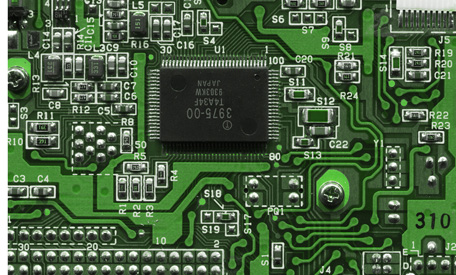
\includegraphics[width=3in, height=1.81in]{microchips.jpg}
\end{figure}
\FloatBarrier

\benum
\intermediatesubproblem If we were to build a CI for the true mean HALT score of chips in production that day, should we use the $T$ distribution or the $Z$ distribution to compute the margin of error? Use the tree diagram we did in class for univariate data testing. If we can't do anything, explain why.
\easysubproblem Draw the distribution of the average HALT score of the SRS to scale as best you can. Indicate where $\mu$ is. Calculate the standard error. Label the x-axis with numbers to the second decimal place. Indicate the name of the r.v. whose density you are sketching and how it's distributed. Leave the entire page below your sketch blank as we will be using it later in the question.
\easysubproblem If the chips have a different HALT score than 7, then the plant has a big problem and they should investigate. The cost of not finding a problem is much higher than the cost of shutting down and investigating. Frame this statement in terms of Type I and II errors and explain why $\alpha$ should be picked high or low.

\easysubproblem Regardless of the $\alpha$ you picked, let $\alpha = 10\%$ since we want to be conservative. Indicate the cutoff point(s) for $\xbar$ and lightly shade in the ``rejection'' region in the sketch in part (b).
\easysubproblem Now, we will be simulating a day's sample. We can do this via the following code:

\begin{verbatim}
samp = rnorm(40, 7, 4); 
samp; 
#end placeholder
\end{verbatim}

Copy and past this into \texttt{R}. It should show you the 50 measurements in the sample on the screen. Now, run the following code to get the average of the sample:

\begin{verbatim}
mean(samp);
#end placeholder
\end{verbatim}

The number on the screen is $\xbar$. Find the 90\% confidence margin of error. Write this number down separately as it will be useful for later.

\hardsubproblem What is the $\prob{\mu \in \text{CI}_{\mu, 90\%}}$ where $\text{CI}_{\mu, 90\%}$ is the confidence interval from part (e) which you did not have to compute.

\easysubproblem Before we do another day's SRS and build another confidence interval, what is the $\prob{\mu \in \text{CI}_{\mu, 90\%}}$? In this case, $\text{CI}_{\mu, 90\%}$ refers to the \textit{future} confidence interval from tomorrow's experiment, not the one we built in part (e).

\intermediatesubproblem Now, we're going to get samples for many days. Since we only care about inference for $\mu$, we're going to trash the actual data\footnote{If you're interested in why we can just ``trash'' the rest of the data, this is because $\xbar$ is a \textit{sufficient statistic} for $\mu$, something you'll learn about when you take Stat 434 with Professor Ewens.} and only look at its average, $\xbar$. Run the following code 25 times in a row:\footnote{use the $\uparrow$ key on your keyboard in the \texttt{R} console and press enter to make this go faster.}

\begin{verbatim}
mean(rnorm(40, 7, 4));
#end placeholder
\end{verbatim}

For each draw (or realization) of $\xbar$ from $\Xbar$, build a 90\% CI. Draw each of these 25 CI's using a line segment below the sketch from part (a).

\easysubproblem Now extend the line of $\mu$ and count the number of CI's that do \textit{not} include $\mu$. This is a duplication of the graphic that appears on p.361 of S\&F. Does the count of these unlucky CI's make sense given our $\alpha$ level?

\hardsubproblem Calculate the probability you take 25 SRS's and have this many CI's not capture $\mu$.

\easysubproblem Consider the more likely case that we do not know the true standard deviation $\sigma$. Can we build a confidence interval for the true mean HALT score?

\easysubproblem Assume HALT scores are normally distributed. Take another SRS and compute $\xbar$ and $s$ by running the following code to get $\xbar$ and $s$:

\begin{verbatim}
samp = rnorm(40, 7, 4);
mean(samp);
sd(samp);
#end placeholder
\end{verbatim}

Build a 99\% CI for $\mu$ for the sample above and notate it like we do in class.

  
\eenum

\problem We take a survey to see if people will buy a piece of software. The product costs \$10. We do many different surveys. They all consist of asking $n$ users who come across the homepage and ask them if they would buy the service:

\beqn
\text{Survey 1}: &n=200,& 36 ~\text{people say yes} \\
\text{Survey 2}: &n=400,& 67 ~\text{people say yes} \\
\text{Survey 3}: &n=800,& 121 ~\text{people say yes} \\
\text{Survey 4}: &n=1600,& 265 ~\text{people say yes} \\
\text{Survey 5}: &n=3200,& 501 ~\text{people say yes} \\
\eeqn 

\begin{figure}[htp]
\centering

\includegraphics[width=2.5in,height=1.65in]{survey.jpg}
\end{figure}
\FloatBarrier

\benum
\easysubproblem Are any of the above good surveys if our goal is to make inference about the proportion of people who will buy the product online?

\easysubproblem Build a 95\% CI for the proportion of people who will buy this product when it is released using each of the above surveys.

\hardsubproblem If we're comfortable with this margin of error on survey 1, allow the margin of error to remain constant for surveys 2, 3, 4, and 5. What will the coverage probabilities be for each survey?

\easysubproblem Can we build a 95\% CI for the number of people that will buy the product when it is released? Explain why or why not.

\easysubproblem Can we build a 95\% CI for the amount of revenue the company will make when the product is released? Explain why or why not.

\easysubproblem Using survey 3, provide a confidence interval for the \textit{number of people} who subscribe for one month if 100,000 people visit the homepage in one year.

\easysubproblem Using survey 3 and the previous question, provide a confidence interval for the year's revenue in euros. Assume everyone subscribes and pays up front for one month. Use the exchange rate \$1 = \EURcr 0.70.

\hardsubproblem Last year the company had revenues of \$120,000. Create a 95\% CI for the \textit{percentage change} in revenue. You may want to reread pp. 362-364.

\eenum

\paragraph{One-proportion and one-sample hypothesis testing} These questions are going to familiarize you with the methodology of univariate hypothesis testing and introduce you to a basic power calculation. \\

\problem You are running the craps tables at the casino.

\begin{figure}[htp]
\centering
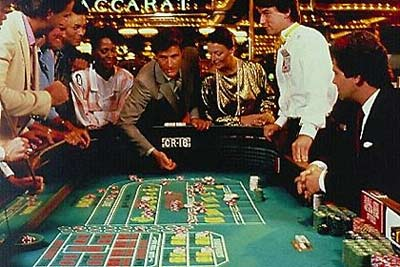
\includegraphics[width=3in,height=2.00in]{craps.jpg}
\end{figure}
\FloatBarrier 

There is someone suspiciously winning. He seems to hardly ever ``crap out'' \ie roll a seven on two dice (the sum of two dice is 7). From table records you see he has rolled 113 rounds (rolls of both dice simultaneously) and only crapped out 13 times. He then left the casino with a large bundle of winnings and you face the decision whether or not to let him back in next time.

\benum
\intermediatesubproblem Frame this as a hypothesis test. Write down $H_0$ and $H_a$. Write it in English first then write the mathematical statements for the hypotheses.
\easysubproblem Talk about what a Type I error is and what a type II error is in this context.
\easysubproblem What would the costs of each error be?
\intermediatesubproblem You decide to take a middle-of-the-road approach and take an $\alpha = 5\%$. Run the hypothesis test and calculate the $\pval$.
\easysubproblem What is your conclusion? Is the result statistically significant?
\intermediatesubproblem What is your strategy for the future when you see him playing at the craps tables again?
\easysubproblem If this guy really knows how to \href{http://en.wikipedia.org/wiki/Dice_setting}{set the dice} and actually can set so that the proportion of 7's is 11\% which is for an expert dice setter, he can really cheat the casino out of a lot of money at his gambling rate. Set this scenario up as a hypothesis test but do not do any computations.
\hardsubproblem Calculate the power of this test \ie the probability of detecting whether this guy is an expert dice setter.
\hardsubproblem How many rounds do you have to observe this guy before you can detect that he's an expert dice setter with probability 80\%?\footnote{For some reason 80\% is the \href{http://en.wikipedia.org/wiki/Statistical_power}{standard power-level} statisticians use; it is analagous to the standard $\alpha=5\%$.}
\eenum

\problem According to the official Collegeboard 2010 \href{http://professionals.collegeboard.com/profdownload/2010-total-group-profile-report-cbs.pdf}{report}, the mean math score is 516 with SD 112 (see table 1, page 1). Download \texttt{SAT.jmp} which is all the SAT data for the incoming freshmen class of 2008 anonymized.

\begin{figure}[htp]
\centering

\includegraphics[width=3in,height=0.96in]{sat_logo.jpg}
\end{figure}
\FloatBarrier

\benum
\easysubproblem Analyze the distribution of the math scores. Are they normally distributed? Print a Q-Q plot and attach it to your homework.
\easysubproblem It looks like there's a black vertical line in the Q-Q plot. Why is it there? What does it correspond to?
\hardsubproblem JMP displays a diamond in the box and whisker plot to indicate a 95\% CI for the mean. Is JMP's CI exact in this case? Explain.
\easysubproblem SAT math scores are known to be normally distributed. Are the incoming Freshmen class of 2008 an SRS of all students that took the SAT's? Base your answer on the analysis of distribution on the screen in JMP.
\intermediatesubproblem Test that the incoming students have a higher than average math score. Compute a $\pval$. Is this lower than you expected? Think about what the $\pval$ means: is the null hypothesis ridiculous in this context?
\easysubproblem We now examine the $n=43$ homeschooled students of that incoming class. Their SAT math scores are below:

\begin{verbatim}
760 560 690 800 510 800 670 540 730 680 550 800 640 770 420 680 530 
730 560 430 630 560 670 600 800 800 710 530 710 390 660 750 440 610 
660 400 560 800 770 790 330 720 380
\end{verbatim}

We have reason to suggest that they come from a normal distribution but \textit{not} the same distribution as what is published in the SAT 2010 report above. We are interested in testing whether or not they have the same math skills as the average incoming student (as measured by the SAT math examination). Set up a hypothesis test.

\easysubproblem Use JMP to compute a 95\% CI for the mean of Penn-admitted homeschooled student math scores. 
\intermediatesubproblem Carry out the hypothesis test at $\alpha = 5\%$. Use the $\pval$ criterion for acceptance / rejection. Indicate whether or not your result is statistically significant.
\easysubproblem Can you reach the same conclusion you did in part (h) from looking at the CI from part (g)? Why or why not?
\eenum

%do SAT example with two reports 2009 and 2010... show super high stat sign difference but very small actual difference talk about "significant but insignificant" paradox


\paragraph{Contingency tables} This section will introduce you to contingency tables, testing using the $\chi^2$ test for independence, and the concept of lurking variables and Simpson's paradox. \\

\problem We talked about the Berkeley data graduate school admissions data in class. Download the file \texttt{berkeley.JMP} and open it. The data I presented in class was from \href{http://en.wikipedia.org/wiki/Simpson%27s_paradox#Berkeley_gender_bias_case}{Wikipedia}, this data is from another source, so the answers will be a bit different.

\benum

\easysubproblem Define ``observational study''.
\easysubproblem Define ``experiment''.

\begin{figure}[htp]
\centering
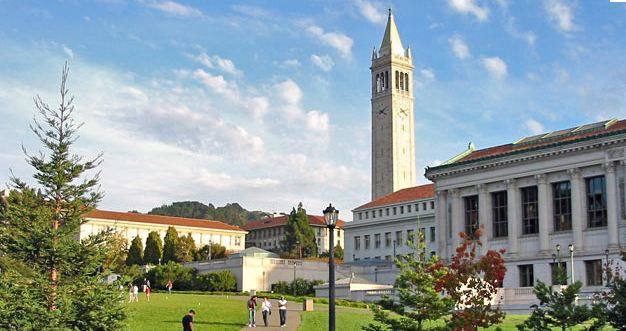
\includegraphics[width=3in,height=2.11in]{berkeley.jpg}
\end{figure}
\FloatBarrier


\easysubproblem Is this Berkeley data the result of an observational study or an experiment and why?
\easysubproblem Use JMP to build a mosaic plot of admission on gender as well as a contingency table (use the ``Fit Y by X'' analysis option). Print both the mosaic plot and the contingency plot and include it with your homework.
\easysubproblem Estimate the probability of being admitted if you're a female. Notate $A$ for ``admitted'' and $F$ for ``female''. Verify your answer with the correct percentage on the contingency table and circle the number(s) on the printout.
\easysubproblem Let $X$ be the r.v. that someone is admitted regardless of gender. How do you model $X$? Which special r.v. do you use? Draw a box around the number(s) on the table you're using to come up with the parameter estimate for such a model.
\easysubproblem We are interested in whether or not gender and the admissions decision are associated. Frame this as a hypothesis test.
\hardsubproblem Execute this test for independence at an $\alpha = 1\%$ confidence level. This will involve building a table of expected counts, calculating a $\chi^2$ test statistic, looking up the correct critical value, making a decision, and writing a sentence of discussion. Your $\chi^2$ statistic should match the ``Pearson'' ``ChiSquare'' in JMP's ``Tests'' panel (don't worry about rounding errors).
\easysubproblem Is it fair to conclude from the previous question that gender and admission decision are associated? Is it fair to conclude that being female or male actually \textit{causes} a prospective candidate to have a larger or smaller chance of being accepted to graduate school at Berkeley?
\intermediatesubproblem Now build a table whose columns are gender and rows are choice of major and whose cells are percentage of applicants admitted. I don't believe that this is an option in JMP (or at least I couldn't figure it out in a reasonable amount of time). I recommend doing a ``Fit Y by X'' where $Y$ is \texttt{admitted?} and $X$ is the interaction \texttt{gender*major} and using the percentages in the contingency table (you will have to figure out which of the three percentages to use).
\easysubproblem Write down the definition of ``lurking variable''. Does major appear to be a lurking variable?
\easysubproblem Write down the definition of ``Simpson's Paradox''. Is the direction of association changing here?
\easysubproblem Write down the definition of ``confounding''.
\intermediatesubproblem Is it possible that there's \textit{another} lurking variable that we haven't controlled for that would flip the direction of association after you control for it in addition to the previous controls?
\eenum

\paragraph{Two-proportion and two-sample hypothesis testing} These questions are going to familiarize you with the methodology of bivariate hypothesis testing: testing interval samples crossed with a nominal variable of two categories. \\

\problem We return to the craps table for another round of gambling. This time, two dice setters are at odds with each other both claiming that they are better than the other. We do an experiment. The first dice setter rolls 224 times and gets 24 sevens; the second dice setter rolls 214 times gets 28 sevens.

\benum
\easysubproblem As a disinterested observer, we want to investigate if there is any statistically significant difference between the two dice setters. Frame this as a hypothesis test.
\intermediatesubproblem Run the test at $\alpha=5\%$, calculate a $\pval$, make a decision, and interpret your results.
\eenum

\problem We return to the SAT data from the \href{http://professionals.collegeboard.com/profdownload/2010-total-group-profile-report-cbs.pdf}{collegeboard report} as well as the SAT data from UPenn admissions.

\benum
\easysubproblem We want to test whether or not men perform better on the critical reading section of the SAT. Frame this as a hypothesis test. 
\intermediatesubproblem Run the test at $\alpha=5\%$. Use the data from p.1 of the report (\ie the page after the table of contents) and assume SAT scores are normally distributed.
\intermediatesubproblem Open \texttt{sat.JMP} again. This time, we want to look at the difference between admitted students' verbal and math scores. In order to do this, we need to combine the \texttt{math} and \texttt{verbal} variables into one variable. Use the \texttt{Tables...Stack} option in the menu. Stack both the \texttt{math} and \texttt{verbal} columns and call the ``Stacked Data Column'' the name ``score'' and the ``Source Label Column'' the name ``mathorverbal''. Upon executing the stack, this should spring up a new data table. Now we can analyze the math vs. verbal side-by-side. Go to ``Fit Y by X''. Enter for $Y$ the variable \texttt{score} and for $X$ the variable  \texttt{mathorverbal}. 

You should now see the bivariate plot with the nominal data on the x-axis and interval data on the y-axis. Click on the red arrow and click ``Quantiles'' to see the box and whisker plot for both the \texttt{math} and \texttt{verbal} datasets. Print this out and attach it to your homework.
\intermediatesubproblem Consider both the \texttt{math} and \texttt{verbal} scores as coming from a normal distribution (even though this seems to be incorrect). Test the difference of these two scores at $\alpha=1\%$.
\easysubproblem Click the red arrow and click ``t Test''. Does your answer from the previous part match JMP's answer?
\eenum 

\end{document}
